\documentclass[10pt,a4paper]{article}
\usepackage[UTF8,fontset = windows]{ctex}
\setCJKmainfont[BoldFont=黑体,ItalicFont=楷体]{华文中宋}
\usepackage{amssymb,amsmath,amsfonts,amsthm,mathrsfs,dsfont,graphicx}
\usepackage{ifthen,indentfirst,enumerate,color,titletoc}
\usepackage{tikz}
\usepackage{multicol}
\usepackage{makecell}
\usepackage{longtable}
\usetikzlibrary{arrows,calc,intersections,patterns,decorations.pathreplacing,3d,angles,quotes,positioning}
\usepackage[bf,small,indentafter,pagestyles]{titlesec}
\usepackage[top=1in, bottom=1in,left=0.8in,right=0.8in]{geometry}
\renewcommand{\baselinestretch}{1.65}
\newtheorem{defi}{定义~}
\newtheorem{eg}{例~}
\newtheorem{ex}{~}
\newtheorem{rem}{注~}
\newtheorem{thm}{定理~}
\newtheorem{coro}{推论~}
\newtheorem{axiom}{公理~}
\newtheorem{prop}{性质~}
\newcommand{\blank}[1]{\underline{\hbox to #1pt{}}}
\newcommand{\bracket}[1]{(\hbox to #1pt{})}
\newcommand{\onech}[4]{\par\begin{tabular}{p{.9\textwidth}}
A.~#1\\
B.~#2\\
C.~#3\\
D.~#4
\end{tabular}}
\newcommand{\twoch}[4]{\par\begin{tabular}{p{.46\textwidth}p{.46\textwidth}}
A.~#1& B.~#2\\
C.~#3& D.~#4
\end{tabular}}
\newcommand{\vartwoch}[4]{\par\begin{tabular}{p{.46\textwidth}p{.46\textwidth}}
(1)~#1& (2)~#2\\
(3)~#3& (4)~#4
\end{tabular}}
\newcommand{\fourch}[4]{\par\begin{tabular}{p{.23\textwidth}p{.23\textwidth}p{.23\textwidth}p{.23\textwidth}}
A.~#1 &B.~#2& C.~#3& D.~#4
\end{tabular}}
\newcommand{\varfourch}[4]{\par\begin{tabular}{p{.23\textwidth}p{.23\textwidth}p{.23\textwidth}p{.23\textwidth}}
(1)~#1 &(2)~#2& (3)~#3& (4)~#4
\end{tabular}}
\begin{document}

\begin{enumerate}[1.]

\item { (000776)}已知集合$A=\{1,3,5,7,9\}$, $B=\{0,1,2,3,4,5\}$, 则图中阴影部分集合用列举法表示的结果是\blank{50}.
\begin{center}
    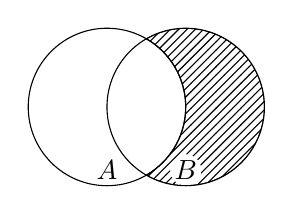
\begin{tikzpicture}
        \begin{scope}[even odd rule]
            \clip  (1,-0.8) circle (0.2) (1,0) circle (1);
            \filldraw [pattern = {north east lines}] (0.5,{0.5*sqrt(3)}) arc (60:-60:1) arc (-120:120:1);
        \end{scope}
        \draw (0,0) circle (1);
        \draw (1,0) circle (1);
        \draw (0,-0.8) node {$A$};
        \draw (1,-0.8) node {$B$};
    \end{tikzpicture}
\end{center}


关联目标:

K0104002B|D01001B|能用文氏图反映两个集合的交集.

K0104007B|D01001B|能用文氏图反映一个集合的补集.



标签: 第一单元

答案: $\{0, 2, 4\}$

解答或提示: 暂无解答与提示

使用记录:

20220510	2022届高三1班	\fcolorbox[rgb]{0,0,0}{1.000,0.000,0}{1.000}


出处: 赋能练习
\item { (002710)}如图, $U$为全集, $M,P,S$是$U$的三个子集, 则阴影部分所表示的集合是\bracket{20}.
\begin{center}
    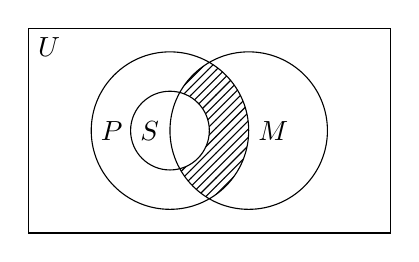
\begin{tikzpicture}
        \begin{scope}
            \clip (1,0) circle (1);
            \begin{scope}[even odd rule]
                \clip (0,0) circle (1) (0,0) circle (0.5);
                \filldraw [pattern = {north east lines}] (-2,-2) rectangle (2,2);
            \end{scope}
        \end{scope}
        \draw (0,0) circle (1) (1,0) circle (1) (0,0) circle (0.5);
        \draw (-1.8,-1.3) rectangle (2.8,1.3);
        \draw (-1.8,1.3) node [below right] {$U$} (-1,0) node [right] {$P$} (-0.5,0) node [right] {$S$} (1,0) node [right] {$M$};
    \end{tikzpicture}
\end{center}
\fourch{$(M\cap P)\cap S$}{$(M\cap P)\cup S$}{$(M\cap P)\cap \overline S$}{$(M\cap P)\cup \overline S$}


关联目标:

K0104002B|D01001B|能用文氏图反映两个集合的交集.

K0104004B|D01001B|能用文氏图反映两个集合的并集.

K0104007B|D01001B|能用文氏图反映一个集合的补集.



标签: 第一单元

答案: C

解答或提示: 暂无解答与提示

使用记录:

20220821	2023届高三2班	\fcolorbox[rgb]{0,0,0}{1.000,0.122,0}{0.939}

20220821	2023届高三3班	\fcolorbox[rgb]{0,0,0}{1.000,0.084,0}{0.958}

20220821	2023届高三10班	\fcolorbox[rgb]{0,0,0}{1.000,0.084,0}{0.958}

20220821	2023届高三9班	\fcolorbox[rgb]{0,0,0}{1.000,0.064,0}{0.968}

20220821	2023届高三12班	\fcolorbox[rgb]{0,0,0}{1.000,0.000,0}{1.000}

20220822	2023届高三10班	\fcolorbox[rgb]{0,0,0}{1.000,0.000,0}{1.000}

20220822	2023届高三8班	\fcolorbox[rgb]{0,0,0}{1.000,0.130,0}{0.935}


出处: 2022届高三第一轮复习讲义
\item { (007702)}用$A$、$B$的运算式表示图中的阴影部分:\\
(1) 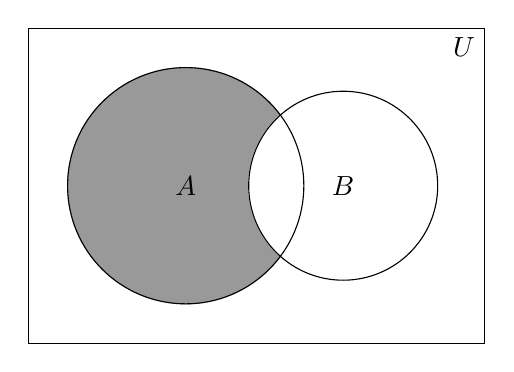
\begin{tikzpicture}
    \filldraw [gray!80] (0,0) circle (1.5);
    \filldraw [white] (2,0) circle (1.2);
    \draw (0,0) circle (1.5) node {$A$} (2,0) circle (1.2) node {$B$};
    \draw (-2,-2) rectangle (3.8,2) node [below left] {$U$};    
\end{tikzpicture} (2) 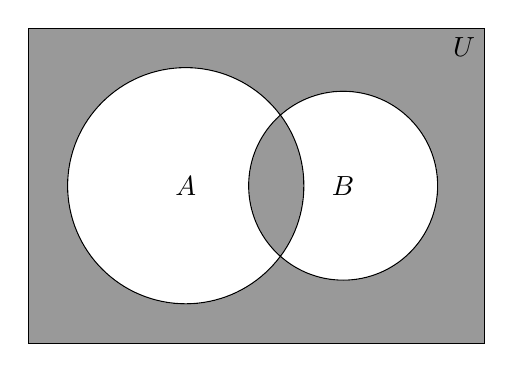
\begin{tikzpicture}
    \filldraw [gray!80] (-2,-2) rectangle (3.8,2);
    \filldraw [even odd rule, white] (0,0) circle (1.5) (2,0) circle (1.2);
    \draw (0,0) circle (1.5) node {$A$} (2,0) circle (1.2) node {$B$};
    \draw (-2,-2) rectangle (3.8,2) node [below left] {$U$};    
\end{tikzpicture}


关联目标:

K0104002B|D01001B|能用文氏图反映两个集合的交集.

K0104004B|D01001B|能用文氏图反映两个集合的并集.

K0104007B|D01001B|能用文氏图反映一个集合的补集.



标签: 第一单元

答案: 暂无答案

解答或提示: 暂无解答与提示

使用记录:

暂无使用记录


出处: 二期课改练习册高一第一学期
\item { (007745)}已知$I$是全集.若$M$、$P$、$S$是$I$的$3$个子集, 则图中阴影部分所表示的集合是\bracket{20}.
\begin{center}
    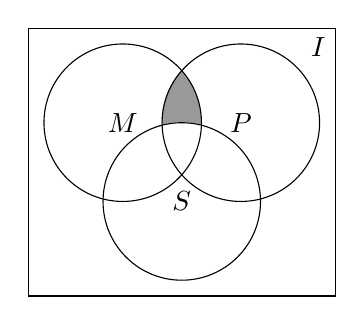
\begin{tikzpicture}
        \begin{scope}
            \clip (0,0) circle (1);
            \filldraw [gray!80] (1.5,0) circle (1);
        \end{scope}
        \filldraw [white] (0.75,-1) circle (1);
        \draw (0,0) circle (1) node {$M$};
        \draw (1.5,0) circle (1) node {$P$};
        \draw (0.75,-1) circle (1) node {$S$};
        \draw (-1.2,-2.2) rectangle (2.7,1.2) node [below left] {$I$};
    \end{tikzpicture}
\end{center}
\fourch{$(M\cap P)\cap S$}{$(M\cap P)\cup S$}{$(M\cap P)\cap \complement _IS$}{$(M\cap P)\cup \complement _IS$}


关联目标:

K0104002B|D01001B|能用文氏图反映两个集合的交集.

K0104007B|D01001B|能用文氏图反映一个集合的补集.



标签: 第一单元

答案: 暂无答案

解答或提示: 暂无解答与提示

使用记录:

暂无使用记录


出处: 二期课改练习册高一第一学期
\item { (020065)}用集合$A$、$B$的运算式表示图中的阴影部分:\\
(1) 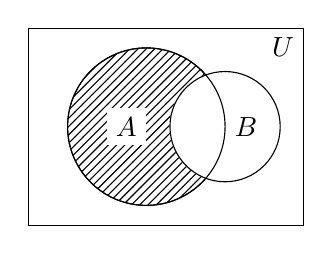
\begin{tikzpicture}
\draw (0,0) rectangle (3.5,2.5) node [below left] {$U$};
\filldraw [pattern = {north east lines}] (1.5,1.25) circle (1);
\filldraw [white] (2.5,1.25) circle (0.7);
\draw (1.5,1.25) circle (1) node [left, fill = white] {$A$};
\draw (2.5,1.25) circle (0.7) node [right] {$B$};
\end{tikzpicture}
(2) 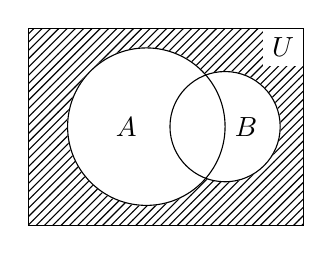
\begin{tikzpicture}
\filldraw [pattern = {north east lines}] (0,0) rectangle (3.5,2.5);
\draw (0,0) rectangle (3.5,2.5) node [below left, fill = white] {$U$};
\filldraw [white] (1.5,1.25) circle (1);
\filldraw [white] (2.5,1.25) circle (0.7);
\draw (1.5,1.25) circle (1) node [left] {$A$};
\draw (2.5,1.25) circle (0.7) node [right] {$B$};
\end{tikzpicture}
(3) 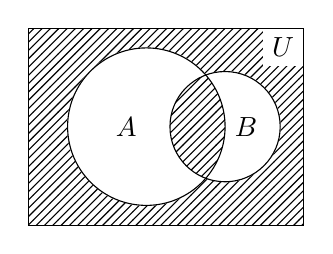
\begin{tikzpicture}
\filldraw [pattern = {north east lines}] (0,0) rectangle (3.5,2.5);
\draw (0,0) rectangle (3.5,2.5) node [below left, fill = white] {$U$};
\filldraw [white] (1.5,1.25) circle (1);
\filldraw [white] (2.5,1.25) circle (0.7);
\begin{scope}
    \clip (1.5,1.25) circle (1);
    \clip (2.5,1.25) circle (0.7);
    \filldraw [pattern = {north east lines}] (0,0) rectangle (3.5,2.5);
\end{scope}
\draw (1.5,1.25) circle (1) node [left] {$A$};
\draw (2.5,1.25) circle (0.7) node [right] {$B$};
\end{tikzpicture}


关联目标:

K0104002B|D01001B|能用文氏图反映两个集合的交集.

K0104004B|D01001B|能用文氏图反映两个集合的并集.

K0104007B|D01001B|能用文氏图反映一个集合的补集.



标签: 第一单元

答案: 暂无答案

解答或提示: 暂无解答与提示

使用记录:

暂无使用记录


出处: 2025届高一校本作业必修第一章
\item { (020069)}如图, 已知集合$U$为全集, 分别用集合$A$、$B$、$C$的运算式表示下列图中的阴影部分.
\begin{center}
    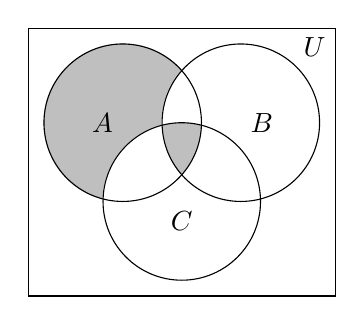
\begin{tikzpicture}
        \filldraw [gray!50] (0,0) circle (1);
        \filldraw [white] (1.5,0) circle (1);
        \filldraw [white] (0.75,-1) circle (1);
        \begin{scope}
            \clip (0,0) circle (1);
            \clip (1.5,0) circle (1);
            \clip (0.75,-1) circle (1);
            \filldraw [gray!50] (1.5,0) circle (1);
        \end{scope}
        \draw (0,0) circle (1) node [left] {$A$};
        \draw (1.5,0) circle (1) node [right] {$B$};
        \draw (0.75,-1) circle (1) node [below] {$C$};
        \draw (-1.2,-2.2) rectangle (2.7,1.2) node [below left] {$U$};
    \end{tikzpicture}
    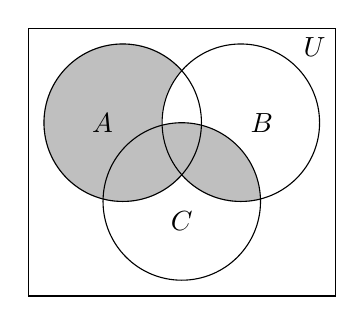
\begin{tikzpicture}
        \filldraw [gray!50] (0,0) circle (1);
        \filldraw [white] (1.5,0) circle (1);
        \begin{scope}
            \clip (0.75,-1) circle (1);
            \filldraw [gray!50] (1.5,0) circle (1);
        \end{scope}
        \draw (0,0) circle (1) node [left] {$A$};
        \draw (1.5,0) circle (1) node [right] {$B$};
        \draw (0.75,-1) circle (1) node [below] {$C$};
        \draw (-1.2,-2.2) rectangle (2.7,1.2) node [below left] {$U$};
    \end{tikzpicture}
\end{center}


关联目标:

K0104002B|D01001B|能用文氏图反映两个集合的交集.

K0104004B|D01001B|能用文氏图反映两个集合的并集.

K0104007B|D01001B|能用文氏图反映一个集合的补集.



标签: 第一单元

答案: 暂无答案

解答或提示: 暂无解答与提示

使用记录:

暂无使用记录


出处: 2025届高一校本作业必修第一章
\item { (030005)}若$M,P$都是全集$U$的子集, 则图中阴影部分可以表示为\bracket{20}
\fourch{$M\cup P$}{$\complement_U(M\cap P)$}{$\complement_UM\cup \complement_UP$}{$\complement_U(M\cup P)$}
\begin{center}
    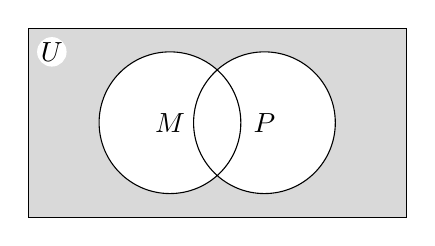
\begin{tikzpicture}[scale = 0.6]
        \filldraw [gray!30] (-3,-2) rectangle (5,2);
        \filldraw [white] (-2.5,1.5) circle (0.3);
        \draw (-2.5,1.5) node {$U$};
        \filldraw [white] (0,0) circle (1.5);
        \filldraw [white] (2,0) circle (1.5);
        \draw (0,0) circle (1.5) node {$M$} (2,0) circle (1.5) node {$P$};
        \draw (-3,-2) rectangle (5,2);
    \end{tikzpicture}
\end{center}


关联目标:

K0104002B|D01001B|能用文氏图反映两个集合的交集.

K0104004B|D01001B|能用文氏图反映两个集合的并集.

K0104007B|D01001B|能用文氏图反映一个集合的补集.



标签: 第一单元

答案: D

解答或提示: 暂无解答与提示

使用记录:

暂无使用记录


出处: 代数精编第一章集合与命题
\end{enumerate}



\end{document}